\normalsize
\section{Gravity Current Test}
\label{section-ANH-Test}

\begin{comment}
10-3 (N.s/m2)   Kinematic Viscosity
- ? -
10-6 (m2/s)

   10-3 (N.s/m2)  10-6 (m2/s)
0   1.787   1.787
5   1.519   1.519
10  1.307   1.307
20  1.002   1.004
30  0.798   0.801
40  0.653   0.658
50  0.547   0.553
60  0.467   0.475
70  0.404   0.413
\end{comment}
This adjustable non-hydrostatics seems to be a simple and practical idea, therefore a numerical model is developed in Chapter \ref{chapter:FlowModel} to test the practicality of this technique. The numerical model is built for incompressible flow simulations in the primitive variables formulation and staggered-grid discretization. This model uses a staggered grid and a modified constrained-interpolated-profile method (Chapter \ref{MCIP}) for transport equation and a successive-over-relaxation solver for the pressure Poisson equation. The numerical simulation has a similar setup to the experiment of gravity current propagation into a linearly stratified fluid demonstrated by Maxworthy et al. \cite{Maxworthy02}, as described in Chapter \ref{chapter:GravityCurrentTest}: A fixed volume of denser fluid at the left boundary of a tank is suddenly released into the ambient fluid with stratification. The tank is 1.4(m) long, 0.2(m) wide, and 0.3(m) deep. The bottom slope is zero. The water depth is 0.15 (m).

The numerical model uses uniform grid spacings of 0.01$(m)$ in $x$, 0.04$(m)$ in $y$, and 0.0025$(m)$ in $z$. The time step ranges from 0.05$(sec)$ to 0.001$(sec)$. The diffusion coefficient of velocity is tested from $10^{-4} (m^2/s)$ to $10^{-6} (m^2/s)$. The density of the fluid is computed from the simplified equation of state \cite{Gill1982},
\begin{equation}
\rho = \rho_o +0.75887 \ s
\end{equation}
The temperature is assumed to be constant and is equal to 20 degree Celsius. The pressure is set to 1 atmosphere. The salinity, $s$, is the mass of salt in gram dissolved per thousand gram seawater. The salinity in the fixed volume to be released in the left tank is tested from 135 to 155 $(g/1000g)$. The maximum salinity in the linearly stratified environment fluid is tested from 40 to 80 $(g/1000g)$. The diffusivity of salinity is tested from $10^{-4} (m^2/s)$ to $10^{-6} (m^2/s)$.

To quantify the difference between the simulation results of the adjustable non-hydrostatics technique and that of a non-hydrostatic model, the root-mean-square based on the $L^p$ norm is used,
\be
error_p= \left(\f{\sum_{i=1}^{N}|\mathbf{x_i}|^p}{N}\right)^{1/p}
\ee
\be
\mathbf{x_i} = x_i - y_i
\ee
$p=1$ gives the average deviation and $p=2$ gives the root-mean-square:
\be
error_1=\sqrt{\f{\sum_{i=1}^{N} |x_i-y_i|}{N}}
\ee
\be
error_2=\sqrt{\f{\sum_{i=1}^{N} (x_i-y_i)^2}{N}}
\ee

The following tables and figures show the simulation results for a selected case.
The salinity equals $149.63 (g/1000g)$ for the released fixed volume and
decreases from $79.63 (g/1000g)$ to zero for the linearly stratified ambient fluid. The fluid density is set to be 1008$(kg/m^3)$ when the salinity equals zero. The dimension of the fixed released volume is 0.2$(m)$ in $x$, 0.2$(m)$ in $y$ and 0.1$(m)$ in $z$. The diffusion coefficient is set to $10^{-6} (m^2/s)$ for velocity and $10^{-5} (m^2/s)$ for salinity. The computational time step is $0.001875 (sec)$.

Table \ref{tab:ANH-summary-2D} and \ref{tab:ANH-summary-3D} show the stopping criteria and the resulting average number of SOR iterations and computation times. It's expected that more stringent requirement results in higher average iteration numbers and longer computation time. Figure \ref{fig:ANH-summary-2D} and \ref{fig:ANH-summary-3D} show the corresponding gravity current simulation plots. It's also concluded in
Table \ref{tab:ANH-hydro-error}-\ref{tab:ANH-E-1SOR20-error}
that the more averaged SOR iterations results in smaller
time-averaged root-mean-square errors\footnote[1]{this error is based on the results of a full hydrodynamic pressure computation that satisfies the maximum velocity divergence ($1/sec$) of $\di \+u<10^{-3}$}.

\cp

\begin{table}[h]%[hbtp]
\vspace{0.6in}
\caption{Two dimensional simulations. SOR iterations for the solution of non-hydrostatic pressure with different stopping criteria.}
\vspace{0.2in}
\small
\begin{center}
\begin{tabular}{ccccc} \hline
\multicolumn{3}{c}{NH pressure computation criteria}  & Ave. SOR Iterations & CPU time (sec) \\ \hline
\multicolumn{3}{c}{Hydrostatic}                                 &  0  &   443.    \\
$\di \mathbf{u} \leq 10^{-1}$ & and & SOR Iterations $\geq 5  $ & 16. &   818.    \\
$\di \mathbf{u} \leq 10^{-1}$ & and & SOR Iterations $\geq 10$  & 24. &   905.    \\
$\di \mathbf{u} \leq 10^{-1}$ & and & SOR Iterations $\geq 20$  & 53. &   1691.     \\
\multicolumn{3}{c}{$\di \mathbf{u} \leq 10^{-3}$}   & 89.  &   2542.     \\ \hline
\end{tabular}
\end{center}
\label{tab:ANH-summary-2D}
\end{table}



\begin{table}[h]%[hbtp]
\vspace{1.2in}
\caption{Three dimensional simulations. SOR iterations for the solution of non-hydrostatic pressure with different stopping criteria.}
\vspace{0.2in}
\small
\begin{center}
\begin{tabular}{ccccc} \hline
\multicolumn{3}{c}{NH pressure computation criteria}  & Ave. SOR Iterations & CPU time (sec) \\ \hline
$\di \mathbf{u} < 10^{-1}$ &and& SOR Iterations $\geq 5  $      &6.   &1946.\\
$\di \mathbf{u}<5 \times 10^{-2}$ &and& SOR Iterations $\geq 5$ &17.  &2749.\\
$\di \mathbf{u} < 10^{-2}$ &and& SOR Iterations $\geq 5$        &54.  &5483.\\
\multicolumn{3}{c}{$\di \mathbf{u} < 10^{-3}$}                  &137. &11495.\\ \hline
\end{tabular}
\end{center}
\label{tab:ANH-summary-3D}
\end{table}

\cp

\begin{figure}[htb]
\vspace{-0.2in}
\subfigure[Hydrostatic]
  { 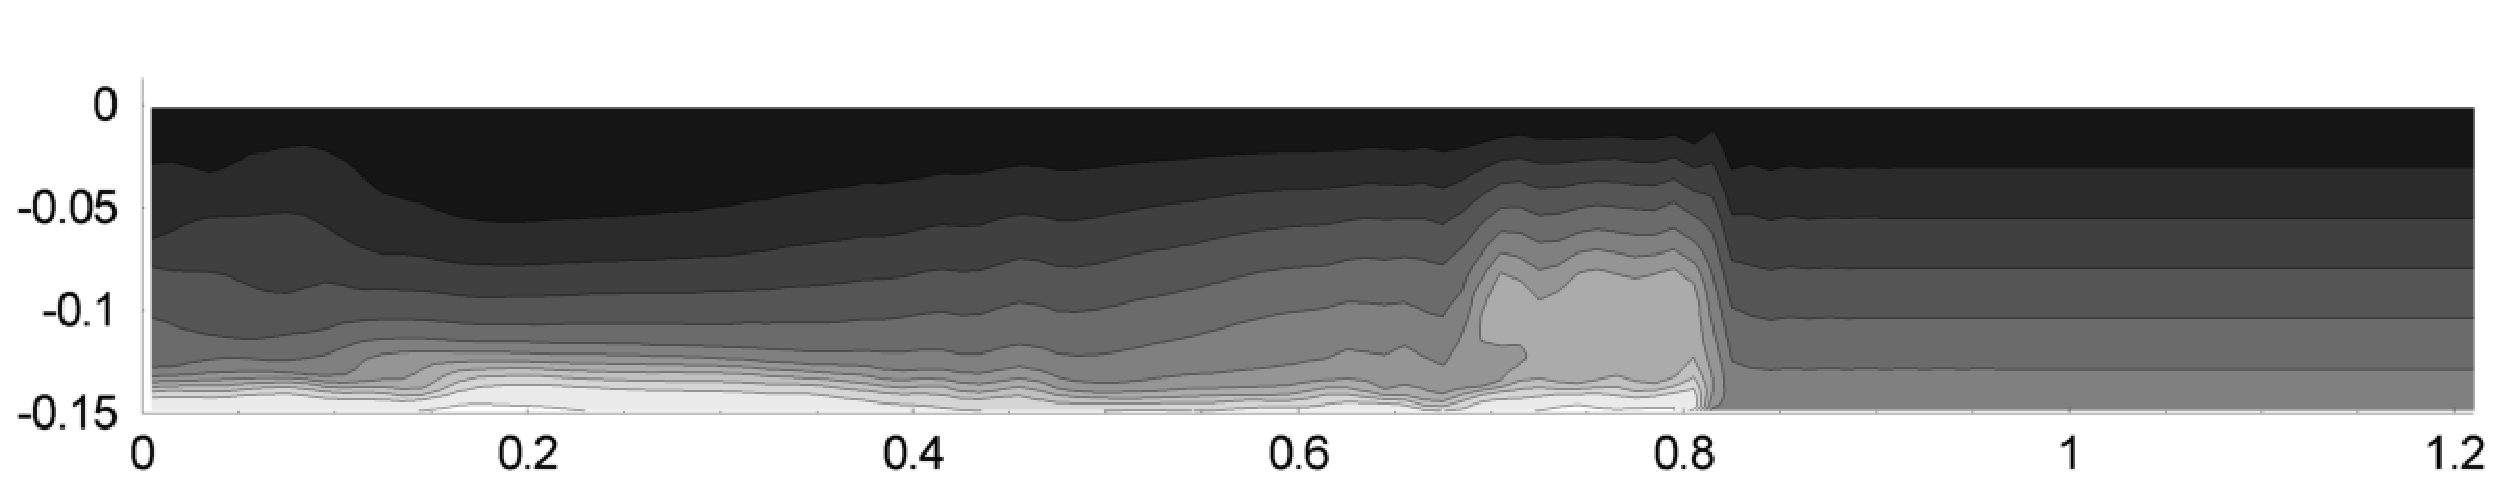
\includegraphics[width=5.6in]{../figures/ANH/2D_NX140/hydro.pdf} }
\subfigure[Maximum Error of Divergence $\leq10^{-1}$ and SOR iterations $\geq 5$]
  { 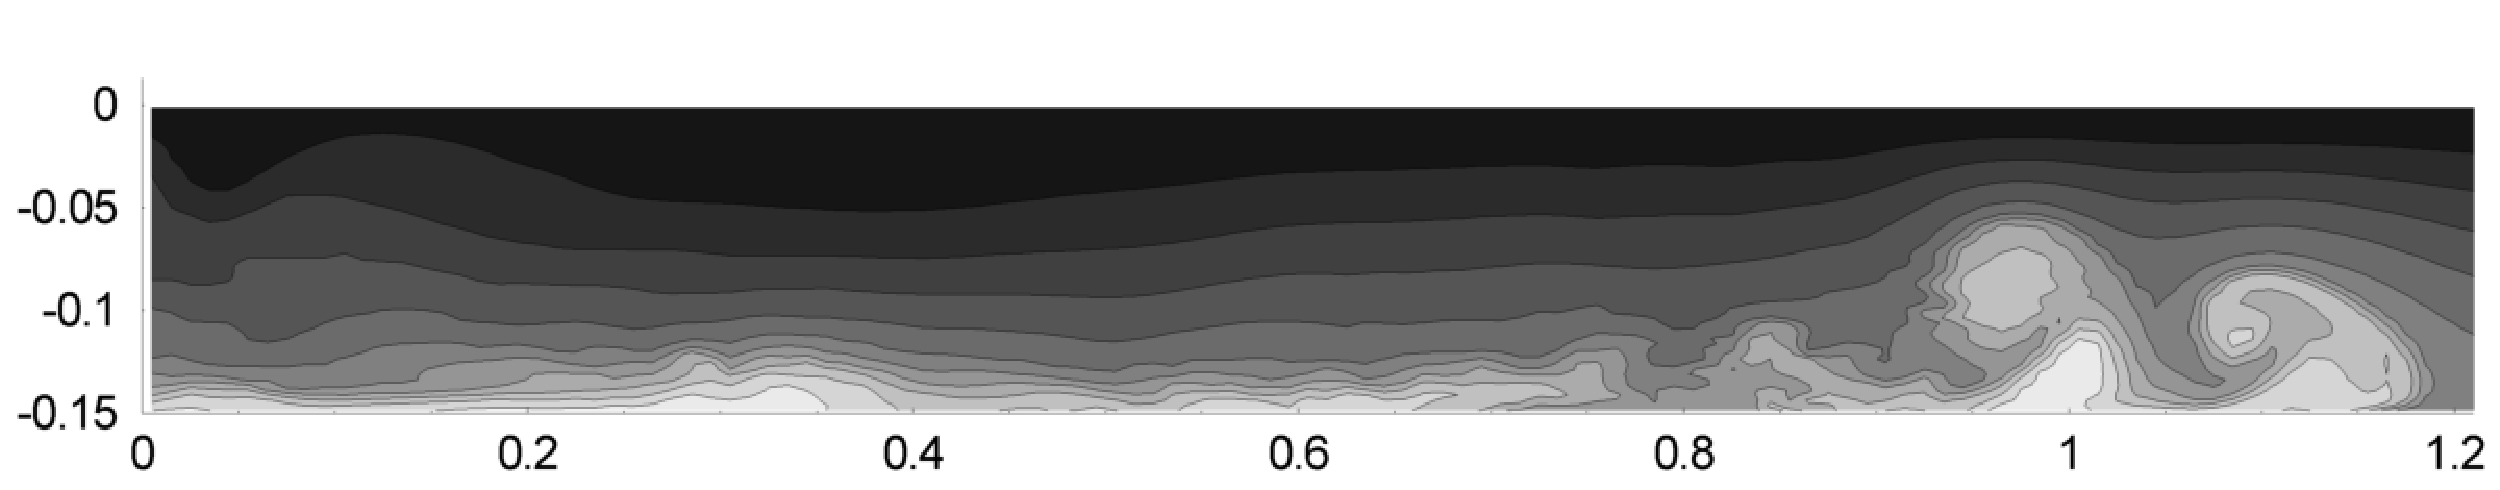
\includegraphics[width=5.6in]{../figures/ANH/2D_NX140/E1SOR5.pdf} }
\subfigure[Maximum Error of Divergence $\leq10^{-1}$ and SOR iterations $\geq 10$]
  { 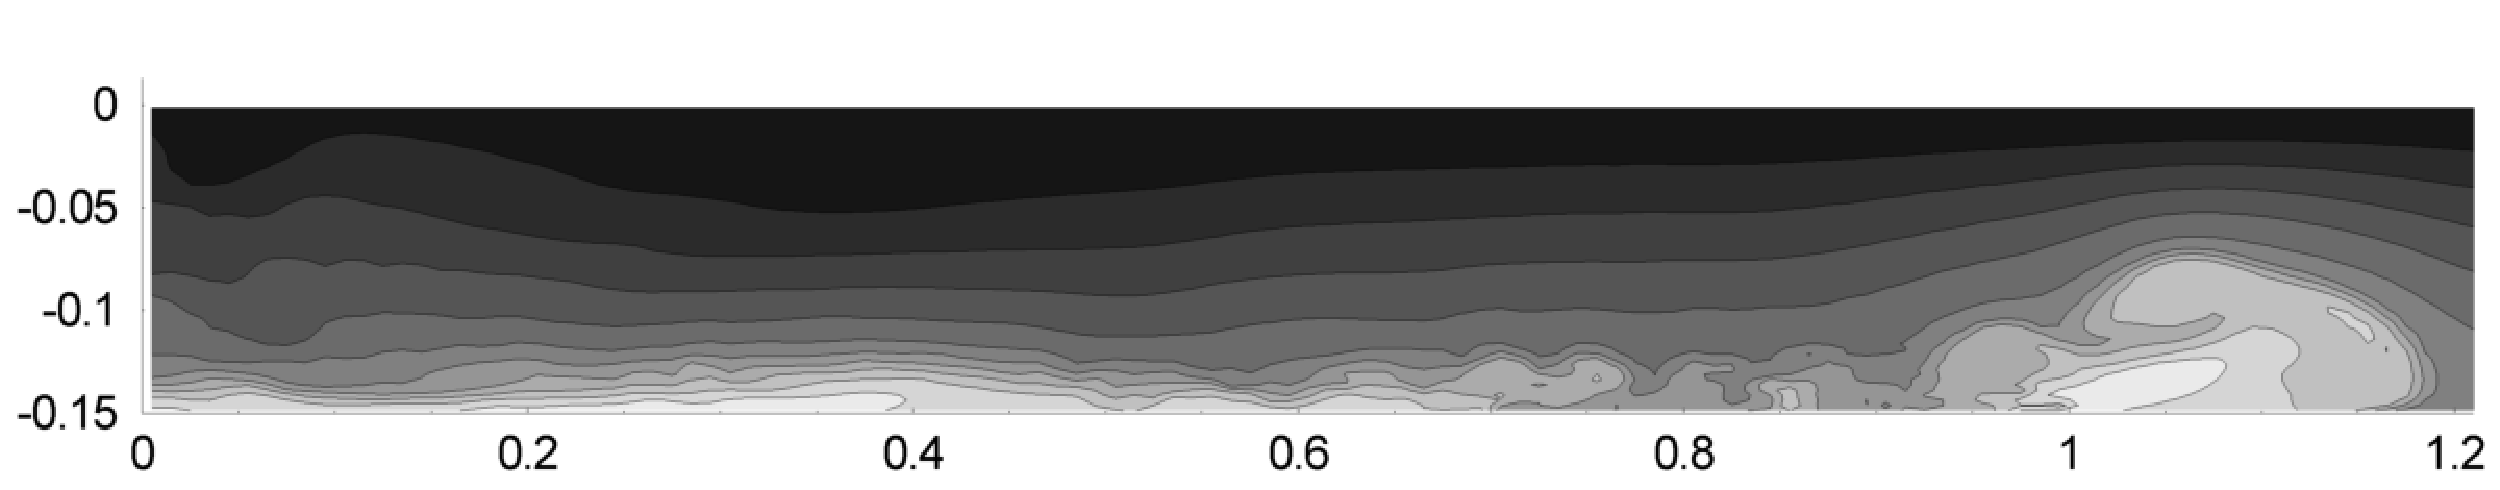
\includegraphics[width=5.6in]{../figures/ANH/2D_NX140/E1SOR10.pdf} }
\subfigure[Maximum Error of Divergence $\leq10^{-1}$ and SOR iterations $\geq 20$]
  { 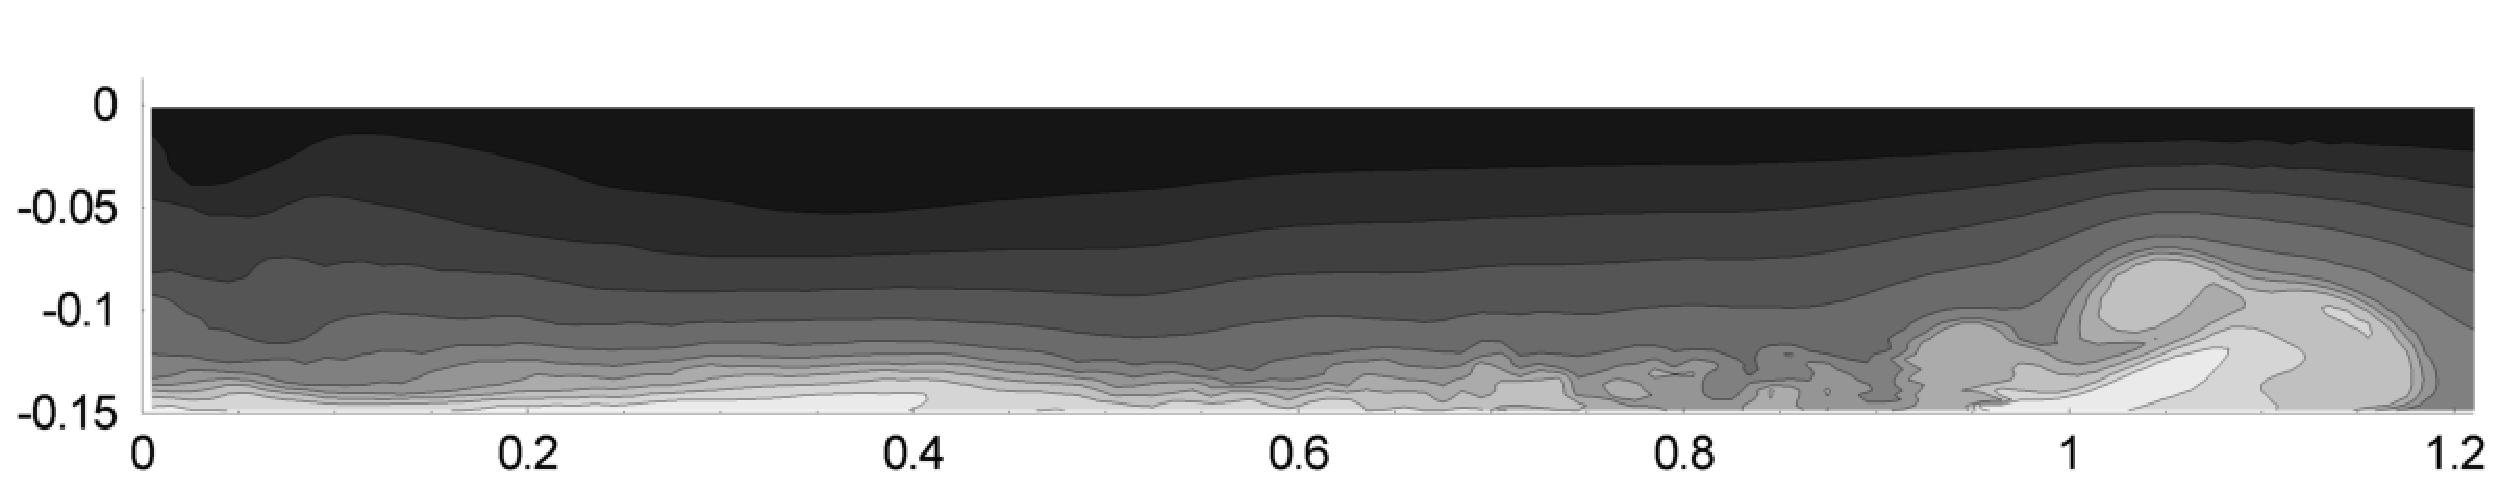
\includegraphics[width=5.6in]{../figures/ANH/2D_NX140/E1SOR20.pdf} }
\subfigure[Maximum Error of Divergence $\leq10^{-3}$]
  { 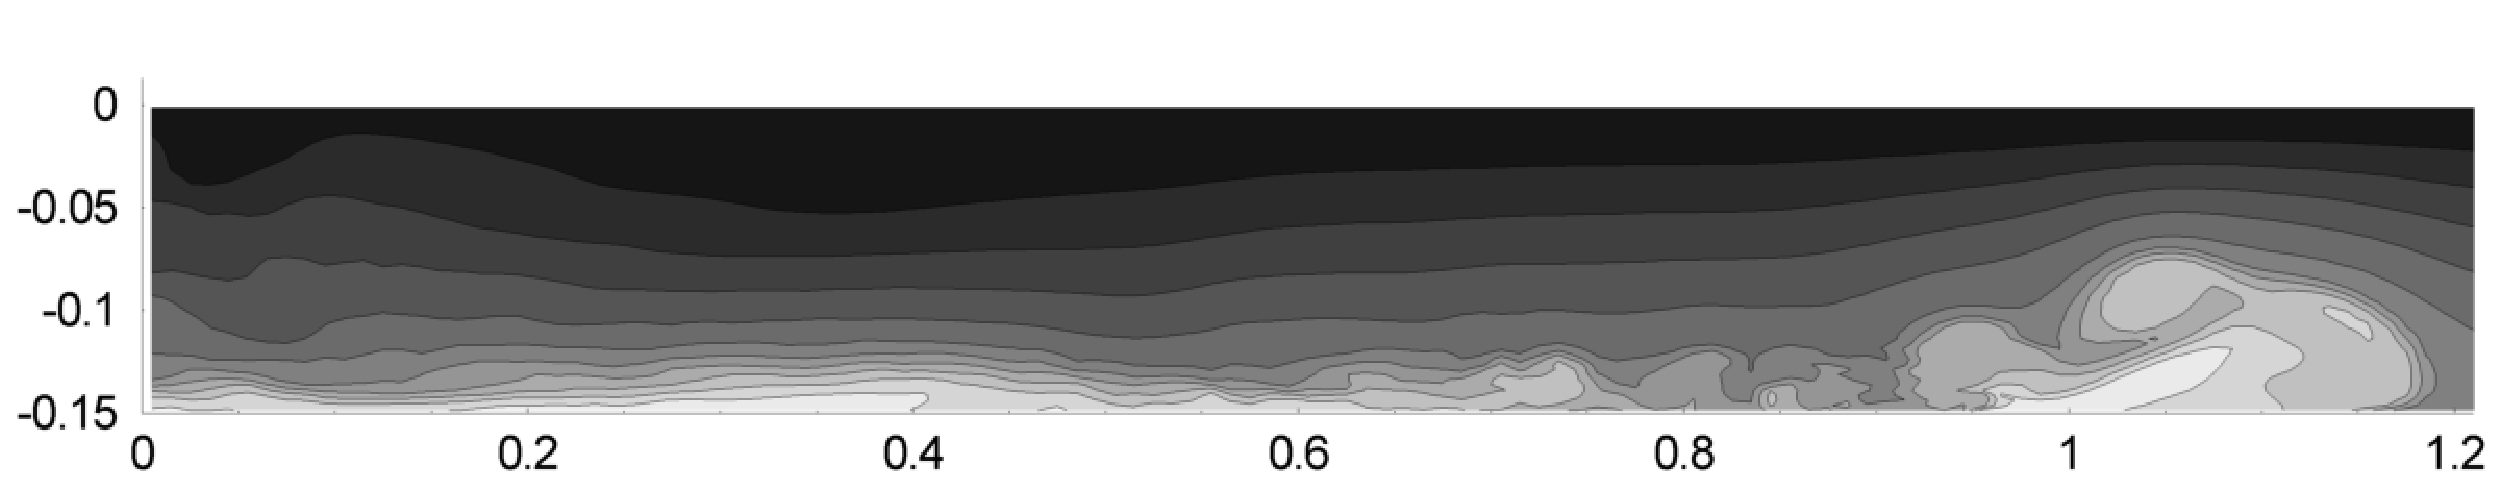
\includegraphics[width=5.6in]{../figures/ANH/2D_NX140/E3.pdf} }
\caption{Two dimensional gravity current simulations at $t = 7.2 (sec)$ for different stopping criteria of SOR iterations for the non-hydrostatic pressure solution}
\label{fig:ANH-summary-2D}
\end{figure}

\begin{figure}[htb]
\hspace{0.0in}
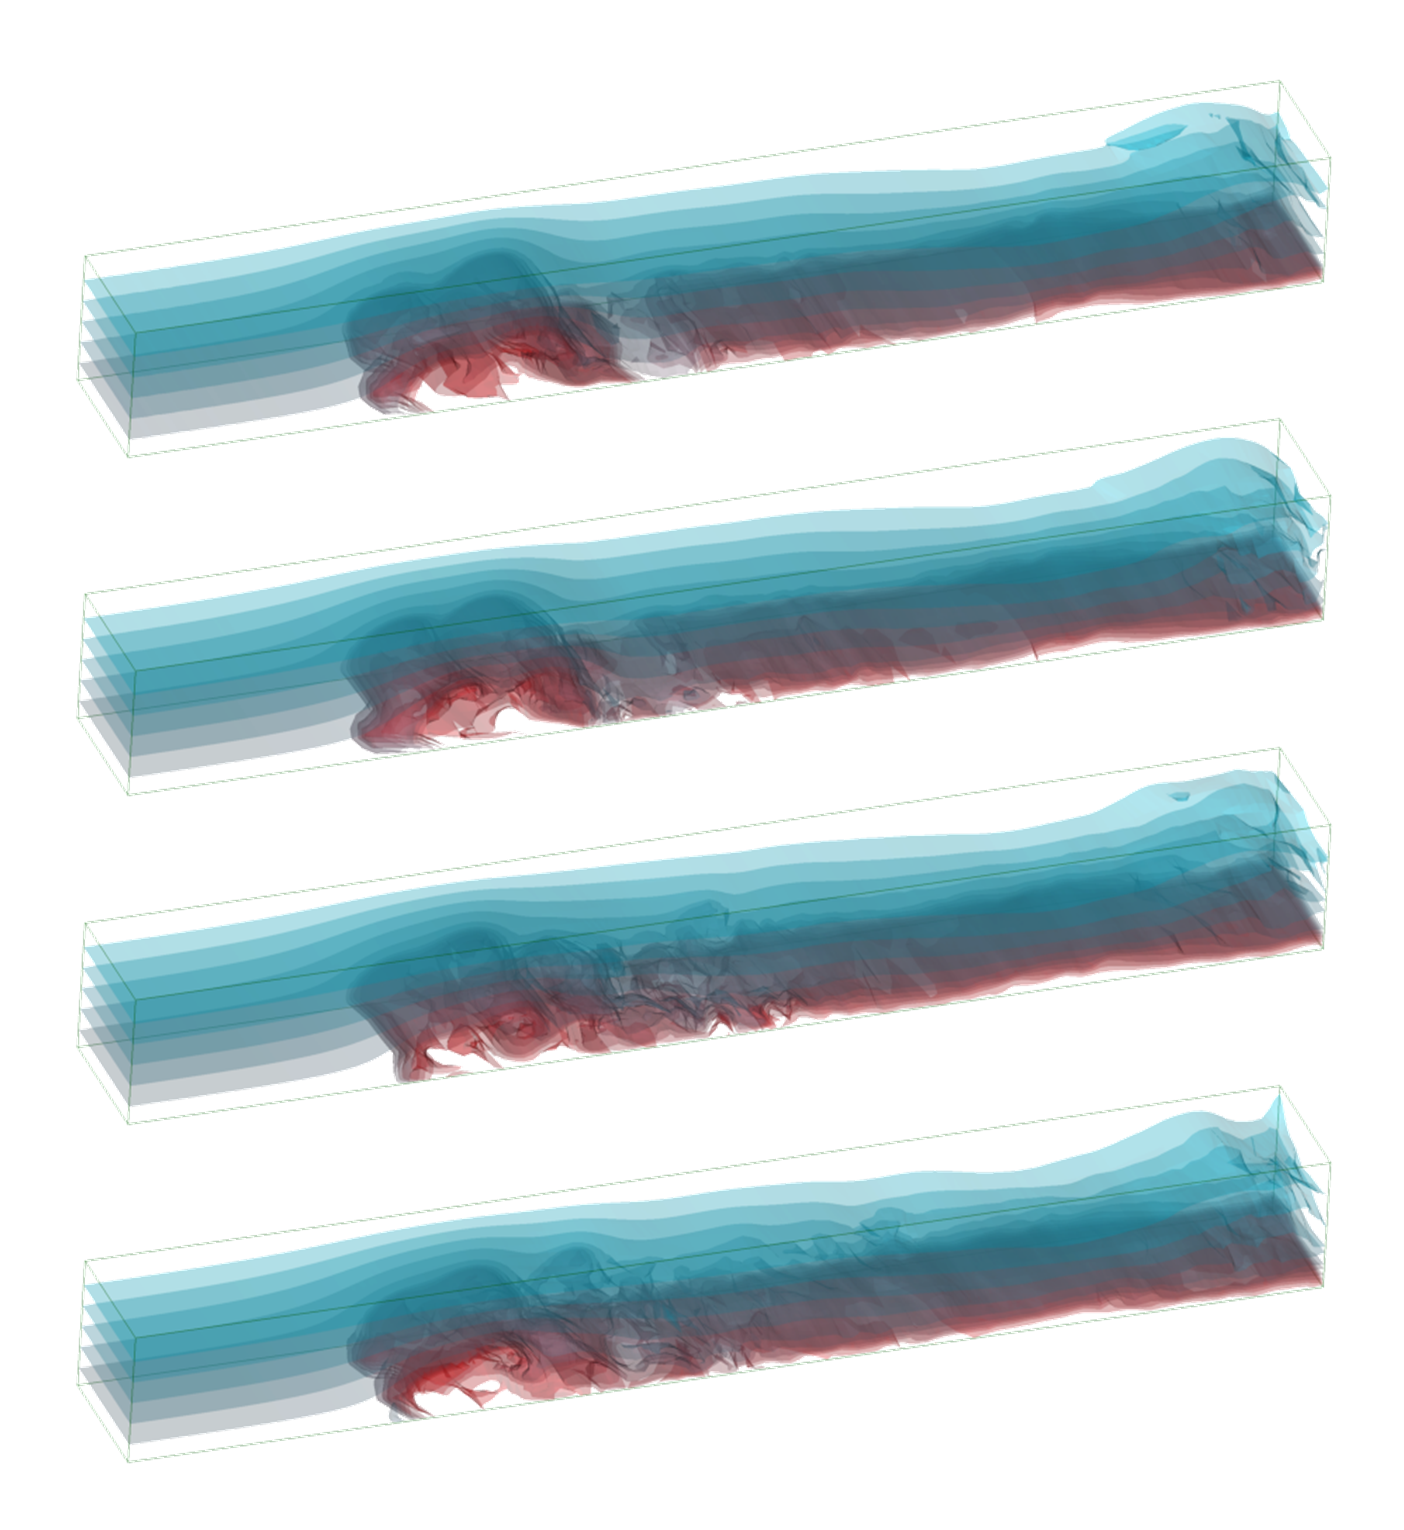
\includegraphics[width=5.8in]{../figures/ANH/3D/ANH-3D.pdf}
\caption{Three dimensional gravity current simulations at $t = 6.3 (sec)$ for different stopping criteria of SOR iterations for the non-hydrostatic pressure solution.
From top to bottom:
(1)$\di \mathbf{u} < 10^{-1}$ and SOR Iterations $\geq 5  $;
(2)$\di \mathbf{u} < 10^{-1}$ and SOR Iterations $\geq 10  $;
(3)$\di \mathbf{u} < 10^{-1}$ and SOR Iterations $\geq 20  $;
(4)$\di \mathbf{u} < 10^{-3}$.}
\label{fig:ANH-summary-3D}
\end{figure}

These tests are performed using a 3.0GH Pentium IV PC with 2GB memory, running windows XP and Intel Fortran compiler version 9.0.029. Five runs of the Linpack benchmark \cite{Dongarra2006} in Java is shown in Table \ref{tab:Linpack Benchmark}.

\begin{table}[h]%[hbtp]
\vspace{0.8in}
\caption{Linpack benchmark \cite{Dongarra2006}}
\vspace{0.2in}
\small
\begin{center}
\begin{tabular}{cccc} \hline
Mflop/s & Time(secs) &  Norm Res &  Precision \\ \hline
167.667 & 0.5        &    5.68   &  2.220446049250313E-16 \\
172.852 & 0.49       &    -   &  - \\
173.209 & 0.48       &    -   &  - \\
178.749 & 0.47       &    -   &  - \\
179.131 & 0.47       &    -   &  - \\ \hline
\end{tabular}
\end{center}
\label{tab:Linpack Benchmark}
\end{table}

\cp
\begin{center}

\begin{table}[h]%[hbtp]
\vspace{1in}
\caption{Two dimensional gravity current simulation with hydrostatic assumption}
\scriptsize
%\hspace{-0.6in}
\begin{tabular}{cccccccccccc} \hline
\multicolumn{12}{c}{ \begin{tabular}{cccccccccc}
$\de t$(sec)  & $\de x$(m) & $\de z$(m) & $CFL_u$ & $CFL_w$ & &  &  & Ave. Iterations & CPU(sec)\\ \hline
0.001875& 0.01 & 0.0025 &0.039 & 0.330 & &         &  &   0. &  443.
\end{tabular} } \\ \hline \hline
 & \multicolumn{3}{c}{density (kg/m3)} & & \multicolumn{3}{c}{u (m/sec)} & & \multicolumn{3}{c}{w (m/sec)}   \\
 \cline{2-4} \cline{6-8} \cline{10-12}
time & $error_2$ &  min & max & & $error_2$ & min & max & & $error_2$ & min & max \\ \hline
    0.4500 &   7.19E+0 &   1.01E+3 &   1.12E+3 &  &   1.30E-2 &  -6.87E-2 &   1.57E-1 &  &   3.13E-2 &  -2.13E-1 &   3.47E-1 \\
    0.9000 &   9.07E+0 &   1.01E+3 &   1.12E+3 &  &   2.60E-2 &  -7.67E-2 &   1.58E-1 &  &   3.50E-2 &  -1.93E-1 &   4.18E-1 \\
    1.3500 &   1.17E+1 &   1.01E+3 &   1.12E+3 &  &   3.40E-2 &  -8.74E-2 &   1.63E-1 &  &   3.56E-2 &  -1.57E-1 &   4.38E-1 \\
    1.8000 &   1.36E+1 &   1.01E+3 &   1.12E+3 &  &   3.89E-2 &  -1.01E-1 &   1.69E-1 &  &   3.51E-2 &  -1.48E-1 &   4.31E-1 \\
    2.2500 &   1.47E+1 &   1.01E+3 &   1.12E+3 &  &   4.18E-2 &  -1.05E-1 &   1.69E-1 &  &   3.52E-2 &  -1.36E-1 &   3.58E-1 \\
    2.7000 &   1.56E+1 &   1.01E+3 &   1.12E+3 &  &   4.54E-2 &  -1.06E-1 &   1.82E-1 &  &   3.49E-2 &  -1.16E-1 &   3.09E-1 \\
    3.1500 &   1.64E+1 &   1.01E+3 &   1.12E+3 &  &   4.99E-2 &  -1.12E-1 &   1.81E-1 &  &   3.76E-2 &  -1.06E-1 &   3.23E-1 \\
    3.6000 &   1.68E+1 &   1.01E+3 &   1.12E+3 &  &   5.22E-2 &  -1.12E-1 &   1.83E-1 &  &   3.97E-2 &  -1.18E-1 &   3.75E-1 \\
    4.0500 &   1.72E+1 &   1.01E+3 &   1.12E+3 &  &   5.52E-2 &  -1.18E-1 &   1.77E-1 &  &   4.25E-2 &  -1.09E-1 &   4.01E-1 \\
    4.5000 &   1.75E+1 &   1.01E+3 &   1.12E+3 &  &   5.68E-2 &  -1.11E-1 &   1.82E-1 &  &   4.18E-2 &  -1.16E-1 &   3.49E-1 \\
    4.9500 &   1.73E+1 &   1.01E+3 &   1.12E+3 &  &   5.78E-2 &  -1.06E-1 &   1.92E-1 &  &   4.13E-2 &  -1.21E-1 &   3.18E-1 \\
    5.4000 &   1.73E+1 &   1.01E+3 &   1.12E+3 &  &   5.80E-2 &  -1.11E-1 &   1.85E-1 &  &   3.83E-2 &  -1.17E-1 &   3.31E-1 \\
    5.8500 &   1.72E+1 &   1.01E+3 &   1.12E+3 &  &   5.89E-2 &  -1.09E-1 &   1.78E-1 &  &   3.98E-2 &  -1.32E-1 &   3.85E-1 \\
    6.3000 &   1.71E+1 &   1.01E+3 &   1.12E+3 &  &   5.78E-2 &  -1.15E-1 &   1.75E-1 &  &   3.99E-2 &  -1.49E-1 &   3.74E-1 \\
    6.7500 &   1.68E+1 &   1.01E+3 &   1.12E+3 &  &   5.85E-2 &  -1.06E-1 &   1.77E-1 &  &   3.89E-2 &  -1.54E-1 &   2.97E-1 \\
    7.2000 &   1.67E+1 &   1.01E+3 &   1.12E+3 &  &   5.95E-2 &  -1.06E-1 &   1.68E-1 &  &   3.81E-2 &  -1.60E-1 &   3.53E-1 \\
 \hline
Average &  1.51E+1& & & &  4.77E-2& & & &  3.78E-2\\
  \hline
 \end{tabular}
 \label{tab:ANH-hydro-error}
 \end{table}
\end{center}
\cp
\begin{center}
\begin{table}[h]%[hbtp]
\vspace{1in}
\caption{Two dimensional gravity current simulation with SOR iteration stopping criteria of $\di u < 0.1$ and SOR iterations $> 5$}
\scriptsize
%\hspace{-0.6in}
\begin{tabular}{cccccccccccc} \hline
\multicolumn{12}{c}{ \begin{tabular}{cccccccccc}
$\de t$(sec)  & $\de x$(m) & $\de z$(m) & $CFL_u$ & $CFL_w$ & &  &  & Ave. Iterations & CPU(sec)\\ \hline
0.001875& 0.01 & 0.0025 &0.096 & 0.205 & &  &  &  16. &  818.
\end{tabular} } \\ \hline \hline
 & \multicolumn{3}{c}{density (kg/m3)} & & \multicolumn{3}{c}{u (m/sec)} & & \multicolumn{3}{c}{w (m/sec)}   \\
 \cline{2-4} \cline{6-8} \cline{10-12}
time & $error_2$ &  min & max & & $error_2$ & min & max & & $error_2$ & min & max \\ \hline
    0.4500 &   7.04E-1 &   1.02E+3 &   1.12E+3 &  &   1.23E-3 &  -1.21E-1 &   2.14E-1 &  &   1.09E-3 &  -1.28E-1 &   9.74E-2 \\
    0.9000 &   9.53E-1 &   1.01E+3 &   1.12E+3 &  &   2.09E-3 &  -1.31E-1 &   2.30E-1 &  &   1.55E-3 &  -8.70E-2 &   1.05E-1 \\
    1.3500 &   9.93E-1 &   1.01E+3 &   1.12E+3 &  &   2.88E-3 &  -1.17E-1 &   2.36E-1 &  &   2.07E-3 &  -6.96E-2 &   1.03E-1 \\
    1.8000 &   1.29E+0 &   1.01E+3 &   1.12E+3 &  &   4.40E-3 &  -1.23E-1 &   2.45E-1 &  &   3.75E-3 &  -8.24E-2 &   9.75E-2 \\
    2.2500 &   2.31E+0 &   1.01E+3 &   1.12E+3 &  &   6.45E-3 &  -1.26E-1 &   2.56E-1 &  &   5.29E-3 &  -1.22E-1 &   9.65E-2 \\
    2.7000 &   2.89E+0 &   1.01E+3 &   1.12E+3 &  &   8.17E-3 &  -1.18E-1 &   2.68E-1 &  &   6.13E-3 &  -8.84E-2 &   1.04E-1 \\
    3.1500 &   2.88E+0 &   1.01E+3 &   1.12E+3 &  &   8.59E-3 &  -1.21E-1 &   2.84E-1 &  &   6.73E-3 &  -8.97E-2 &   1.07E-1 \\
    3.6000 &   3.30E+0 &   1.01E+3 &   1.12E+3 &  &   1.00E-2 &  -1.31E-1 &   2.78E-1 &  &   9.00E-3 &  -9.36E-2 &   1.01E-1 \\
    4.0500 &   3.72E+0 &   1.01E+3 &   1.12E+3 &  &   1.31E-2 &  -1.44E-1 &   3.05E-1 &  &   1.37E-2 &  -1.15E-1 &   9.90E-2 \\
    4.5000 &   4.61E+0 &   1.01E+3 &   1.12E+3 &  &   1.83E-2 &  -1.42E-1 &   2.94E-1 &  &   1.99E-2 &  -1.40E-1 &   9.83E-2 \\
    4.9500 &   5.14E+0 &   1.01E+3 &   1.12E+3 &  &   1.99E-2 &  -1.36E-1 &   2.88E-1 &  &   2.37E-2 &  -1.26E-1 &   1.03E-1 \\
    5.4000 &   5.74E+0 &   1.01E+3 &   1.12E+3 &  &   2.10E-2 &  -1.41E-1 &   2.80E-1 &  &   2.48E-2 &  -1.50E-1 &   1.23E-1 \\
    5.8500 &   6.25E+0 &   1.01E+3 &   1.12E+3 &  &   2.40E-2 &  -1.48E-1 &   2.71E-1 &  &   2.79E-2 &  -1.51E-1 &   1.63E-1 \\
    6.3000 &   6.96E+0 &   1.01E+3 &   1.12E+3 &  &   2.41E-2 &  -1.54E-1 &   2.49E-1 &  &   2.93E-2 &  -1.41E-1 &   2.10E-1 \\
    6.7500 &   7.50E+0 &   1.01E+3 &   1.12E+3 &  &   3.10E-2 &  -1.53E-1 &   3.84E-1 &  &   3.29E-2 &  -2.31E-1 &   2.15E-1 \\
    7.2000 &   8.76E+0 &   1.01E+3 &   1.12E+3 &  &   4.00E-2 &  -1.86E-1 &   2.89E-1 &  &   3.49E-2 &  -1.54E-1 &   1.82E-1 \\
 \hline
Average &  4.00E+0& & & &  1.47E-2& & & &  1.52E-2\\
  \hline
 \end{tabular}
 \label{tab:ANH-E-1SOR5-error}
 \end{table}
\end{center}
\cp
\begin{center}
\begin{table}[h]%[hbtp]
\vspace{1in}
\caption{Two dimensional gravity current simulation with SOR iteration stopping criteria of $\di u < 0.1$ and SOR iterations $> 10$}
\scriptsize
%\hspace{-0.6in}
\begin{tabular}{cccccccccccc} \hline
\multicolumn{12}{c}{ \begin{tabular}{cccccccccc}
$\de t$(sec)  & $\de x$(m) & $\de z$(m) & $CFL_u$ & $CFL_w$ & &  &  & Ave. Iterations & CPU(sec)\\ \hline
0.001875& 0.01 & 0.0025 &0.190 & 0.264 & &  &  &  27. & 1101.
\end{tabular} } \\ \hline \hline
 & \multicolumn{3}{c}{density (kg/m3)} & & \multicolumn{3}{c}{u (m/sec)} & & \multicolumn{3}{c}{w (m/sec)}   \\
 \cline{2-4} \cline{6-8} \cline{10-12}
time & $error_2$ &  min & max & & $error_2$ & min & max & & $error_2$ & min & max \\ \hline
    0.4500 &   7.64E-2 &   1.02E+3 &   1.12E+3 &  &   1.31E-4 &  -1.25E-1 &   2.15E-1 &  &   1.71E-4 &  -1.25E-1 &   9.97E-2 \\
    0.9000 &   1.66E-1 &   1.01E+3 &   1.12E+3 &  &   2.60E-4 &  -1.34E-1 &   2.28E-1 &  &   3.12E-4 &  -8.42E-2 &   1.06E-1 \\
    1.3500 &   1.61E-1 &   1.01E+3 &   1.12E+3 &  &   4.19E-4 &  -1.21E-1 &   2.34E-1 &  &   3.99E-4 &  -7.10E-2 &   1.01E-1 \\
    1.8000 &   1.76E-1 &   1.01E+3 &   1.12E+3 &  &   5.74E-4 &  -1.22E-1 &   2.46E-1 &  &   5.32E-4 &  -9.38E-2 &   9.52E-2 \\
    2.2500 &   2.87E-1 &   1.01E+3 &   1.12E+3 &  &   8.81E-4 &  -1.23E-1 &   2.54E-1 &  &   8.32E-4 &  -1.16E-1 &   9.55E-2 \\
    2.7000 &   4.17E-1 &   1.01E+3 &   1.12E+3 &  &   1.23E-3 &  -1.10E-1 &   2.78E-1 &  &   1.13E-3 &  -9.65E-2 &   1.02E-1 \\
    3.1500 &   5.08E-1 &   1.01E+3 &   1.12E+3 &  &   1.33E-3 &  -1.15E-1 &   2.89E-1 &  &   1.32E-3 &  -1.07E-1 &   1.16E-1 \\
    3.6000 &   6.73E-1 &   1.01E+3 &   1.12E+3 &  &   1.76E-3 &  -1.28E-1 &   2.62E-1 &  &   1.86E-3 &  -1.25E-1 &   1.16E-1 \\
    4.0500 &   7.50E-1 &   1.01E+3 &   1.12E+3 &  &   2.38E-3 &  -1.31E-1 &   2.80E-1 &  &   2.25E-3 &  -1.36E-1 &   9.70E-2 \\
    4.5000 &   9.36E-1 &   1.01E+3 &   1.12E+3 &  &   3.21E-3 &  -1.35E-1 &   2.83E-1 &  &   2.73E-3 &  -1.42E-1 &   9.41E-2 \\
    4.9500 &   1.14E+0 &   1.01E+3 &   1.12E+3 &  &   3.92E-3 &  -1.27E-1 &   3.24E-1 &  &   3.53E-3 &  -1.58E-1 &   1.10E-1 \\
    5.4000 &   1.42E+0 &   1.01E+3 &   1.12E+3 &  &   4.85E-3 &  -1.28E-1 &   2.81E-1 &  &   4.46E-3 &  -1.11E-1 &   1.13E-1 \\
    5.8500 &   1.53E+0 &   1.01E+3 &   1.12E+3 &  &   7.04E-3 &  -1.27E-1 &   2.98E-1 &  &   6.73E-3 &  -1.37E-1 &   1.26E-1 \\
    6.3000 &   1.91E+0 &   1.01E+3 &   1.12E+3 &  &   8.73E-3 &  -1.41E-1 &   2.91E-1 &  &   9.04E-3 &  -1.56E-1 &   1.54E-1 \\
    6.7500 &   2.09E+0 &   1.01E+3 &   1.12E+3 &  &   1.51E-2 &  -1.38E-1 &   4.21E-1 &  &   1.16E-2 &  -1.54E-1 &   2.40E-1 \\
    7.2000 &   2.83E+0 &   1.01E+3 &   1.12E+3 &  &   2.46E-2 &  -2.08E-1 &   5.64E-1 &  &   1.58E-2 &  -2.49E-1 &   1.60E-1 \\
 \hline
Average &  9.42E-1& & & &  4.78E-3& & & &  3.92E-3\\
  \hline
 \end{tabular}
 \label{tab:ANH-E-1SOR10-error}
 \end{table}
\end{center}


\cp
\begin{center}
\begin{table}[h]%[hbtp]
\vspace{1in}
\caption{Two dimensional gravity current simulation with SOR iteration stopping criteria of $\di u < 0.1$ and SOR iterations $> 20$}
\scriptsize
%\hspace{-0.6in}
\begin{tabular}{cccccccccccc} \hline
\multicolumn{12}{c}{ \begin{tabular}{cccccccccc}
$\de t$(sec)  & $\de x$(m) & $\de z$(m) & $CFL_u$ & $CFL_w$ & &  &  & Ave. Iterations & CPU(sec)\\ \hline
0.001875 & 0.01 & 0.0025 &0.172 & 0.249 & & &  &  53. & 1691.
\end{tabular} } \\ \hline \hline
 & \multicolumn{3}{c}{density (kg/m3)} & & \multicolumn{3}{c}{u (m/sec)} & & \multicolumn{3}{c}{w (m/sec)}   \\
 \cline{2-4} \cline{6-8} \cline{10-12}
time & $error_2$ &  min & max & & $error_2$ & min & max & & $error_2$ & min & max \\ \hline
    0.4500 &   6.61E-2 &   1.02E+3 &   1.12E+3 &  &   3.94E-5 &  -1.26E-1 &   2.15E-1 &  &   1.19E-4 &  -1.24E-1 &   9.94E-2 \\
    0.9000 &   1.43E-1 &   1.01E+3 &   1.12E+3 &  &   9.24E-5 &  -1.35E-1 &   2.27E-1 &  &   3.08E-4 &  -8.44E-2 &   1.06E-1 \\
    1.3500 &   1.37E-1 &   1.01E+3 &   1.12E+3 &  &   2.04E-4 &  -1.21E-1 &   2.35E-1 &  &   3.37E-4 &  -7.24E-2 &   1.01E-1 \\
    1.8000 &   1.20E-1 &   1.01E+3 &   1.12E+3 &  &   3.02E-4 &  -1.23E-1 &   2.46E-1 &  &   3.57E-4 &  -9.47E-2 &   9.48E-2 \\
    2.2500 &   1.30E-1 &   1.01E+3 &   1.12E+3 &  &   3.58E-4 &  -1.23E-1 &   2.54E-1 &  &   4.51E-4 &  -1.16E-1 &   9.54E-2 \\
    2.7000 &   1.89E-1 &   1.01E+3 &   1.12E+3 &  &   4.71E-4 &  -1.09E-1 &   2.79E-1 &  &   4.14E-4 &  -9.60E-2 &   1.02E-1 \\
    3.1500 &   2.13E-1 &   1.01E+3 &   1.12E+3 &  &   5.82E-4 &  -1.15E-1 &   2.89E-1 &  &   5.16E-4 &  -1.03E-1 &   1.14E-1 \\
    3.6000 &   2.61E-1 &   1.01E+3 &   1.12E+3 &  &   7.23E-4 &  -1.29E-1 &   2.62E-1 &  &   6.69E-4 &  -1.21E-1 &   1.17E-1 \\
    4.0500 &   2.91E-1 &   1.01E+3 &   1.12E+3 &  &   8.92E-4 &  -1.30E-1 &   2.77E-1 &  &   7.77E-4 &  -1.36E-1 &   9.70E-2 \\
    4.5000 &   3.46E-1 &   1.01E+3 &   1.12E+3 &  &   1.17E-3 &  -1.34E-1 &   2.77E-1 &  &   9.55E-4 &  -1.40E-1 &   9.34E-2 \\
    4.9500 &   4.87E-1 &   1.01E+3 &   1.12E+3 &  &   1.53E-3 &  -1.22E-1 &   2.82E-1 &  &   1.38E-3 &  -1.46E-1 &   1.08E-1 \\
    5.4000 &   6.91E-1 &   1.01E+3 &   1.12E+3 &  &   2.06E-3 &  -1.27E-1 &   2.74E-1 &  &   1.96E-3 &  -1.09E-1 &   1.17E-1 \\
    5.8500 &   7.79E-1 &   1.01E+3 &   1.12E+3 &  &   3.81E-3 &  -1.30E-1 &   2.87E-1 &  &   2.92E-3 &  -1.51E-1 &   1.22E-1 \\
    6.3000 &   1.25E+0 &   1.01E+3 &   1.12E+3 &  &   5.88E-3 &  -1.43E-1 &   2.73E-1 &  &   4.49E-3 &  -1.65E-1 &   1.42E-1 \\
    6.7500 &   1.54E+0 &   1.01E+3 &   1.12E+3 &  &   1.09E-2 &  -1.39E-1 &   4.06E-1 &  &   5.05E-3 &  -1.56E-1 &   2.01E-1 \\
    7.2000 &   1.71E+0 &   1.01E+3 &   1.12E+3 &  &   1.78E-2 &  -2.46E-1 &   6.93E-1 &  &   6.81E-3 &  -1.96E-1 &   1.62E-1 \\
 \hline
Average &  5.22E-1& & & &  2.93E-3& & & &  1.72E-3\\
  \hline
 \end{tabular}
 \label{tab:ANH-E-1SOR20-error}
 \end{table}
\end{center}
\cp

\begin{figure}[h]
\hspace{0.7in} \vspace{0.3in}
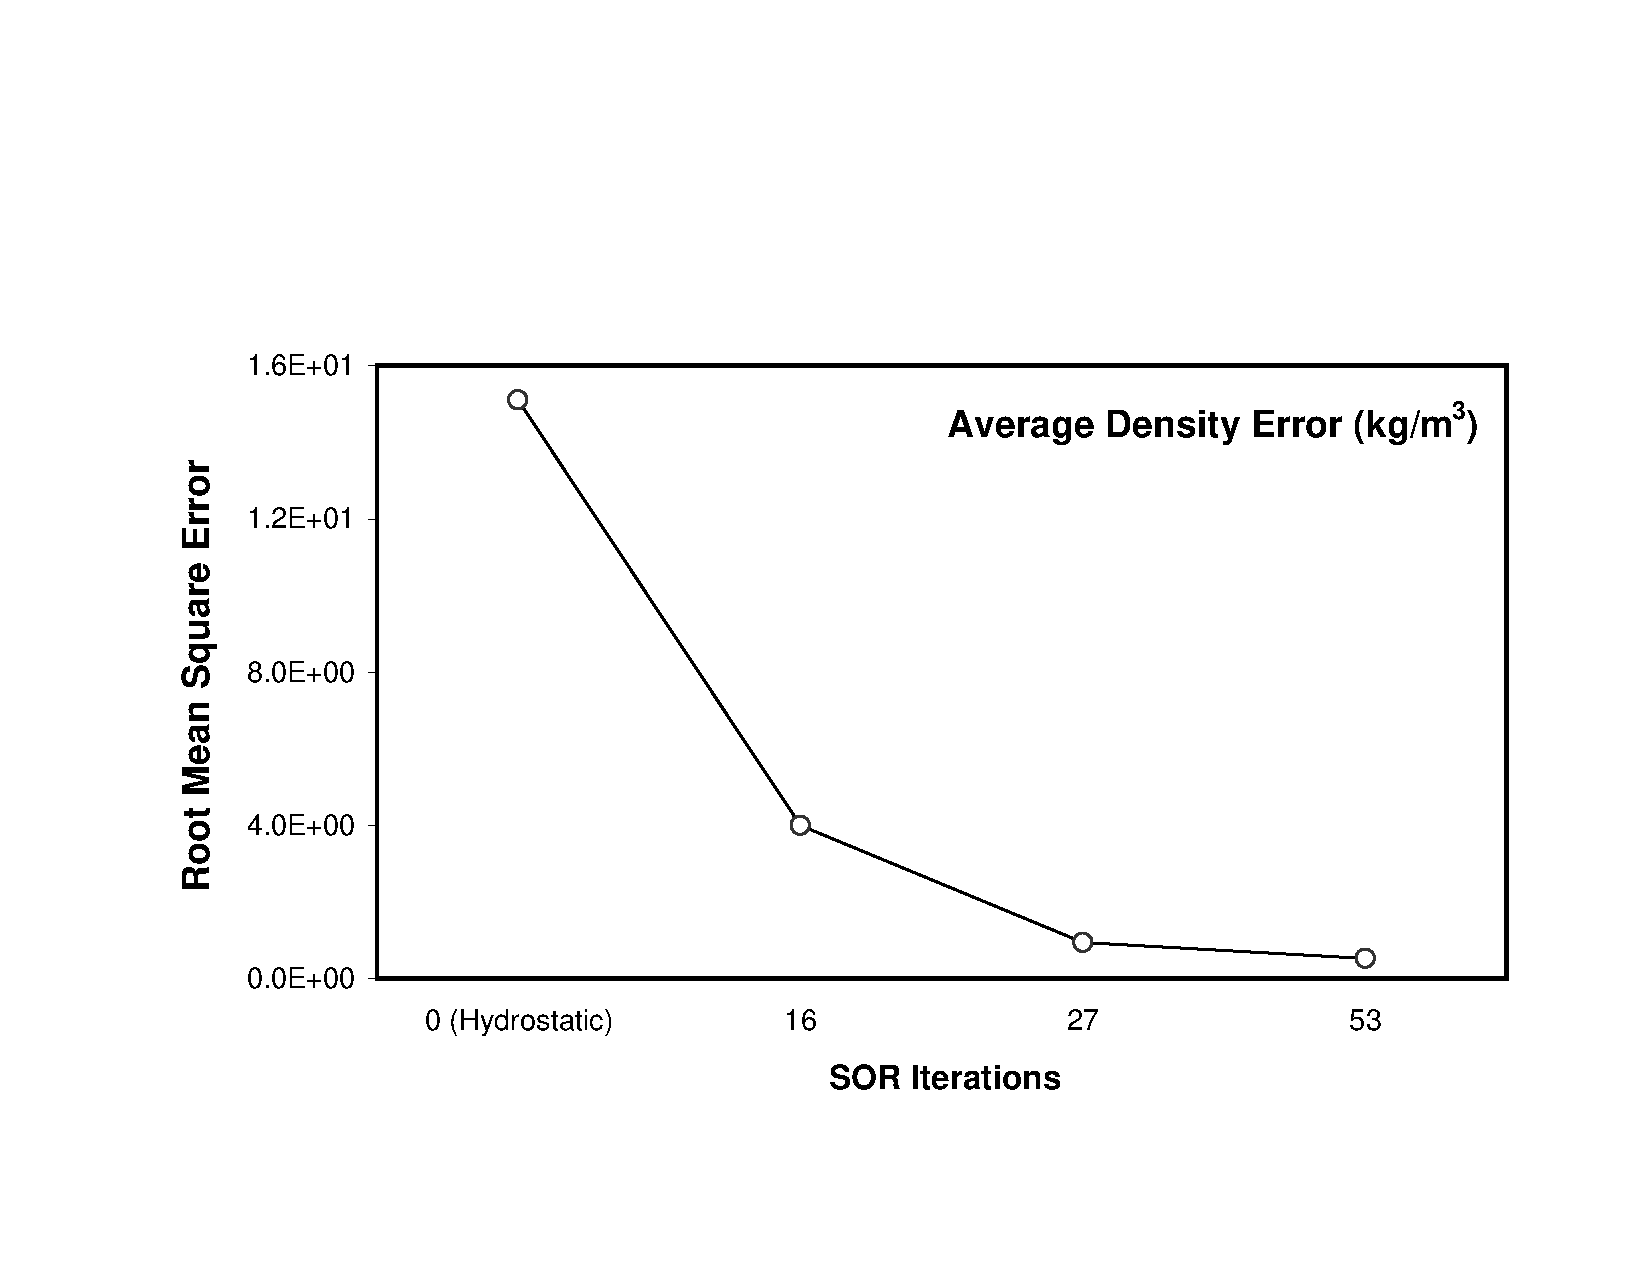
\includegraphics[width=4.0in]{../figures/ANH/2D_NX140/density.pdf}

\hspace{0.7in} \vspace{0.3in}
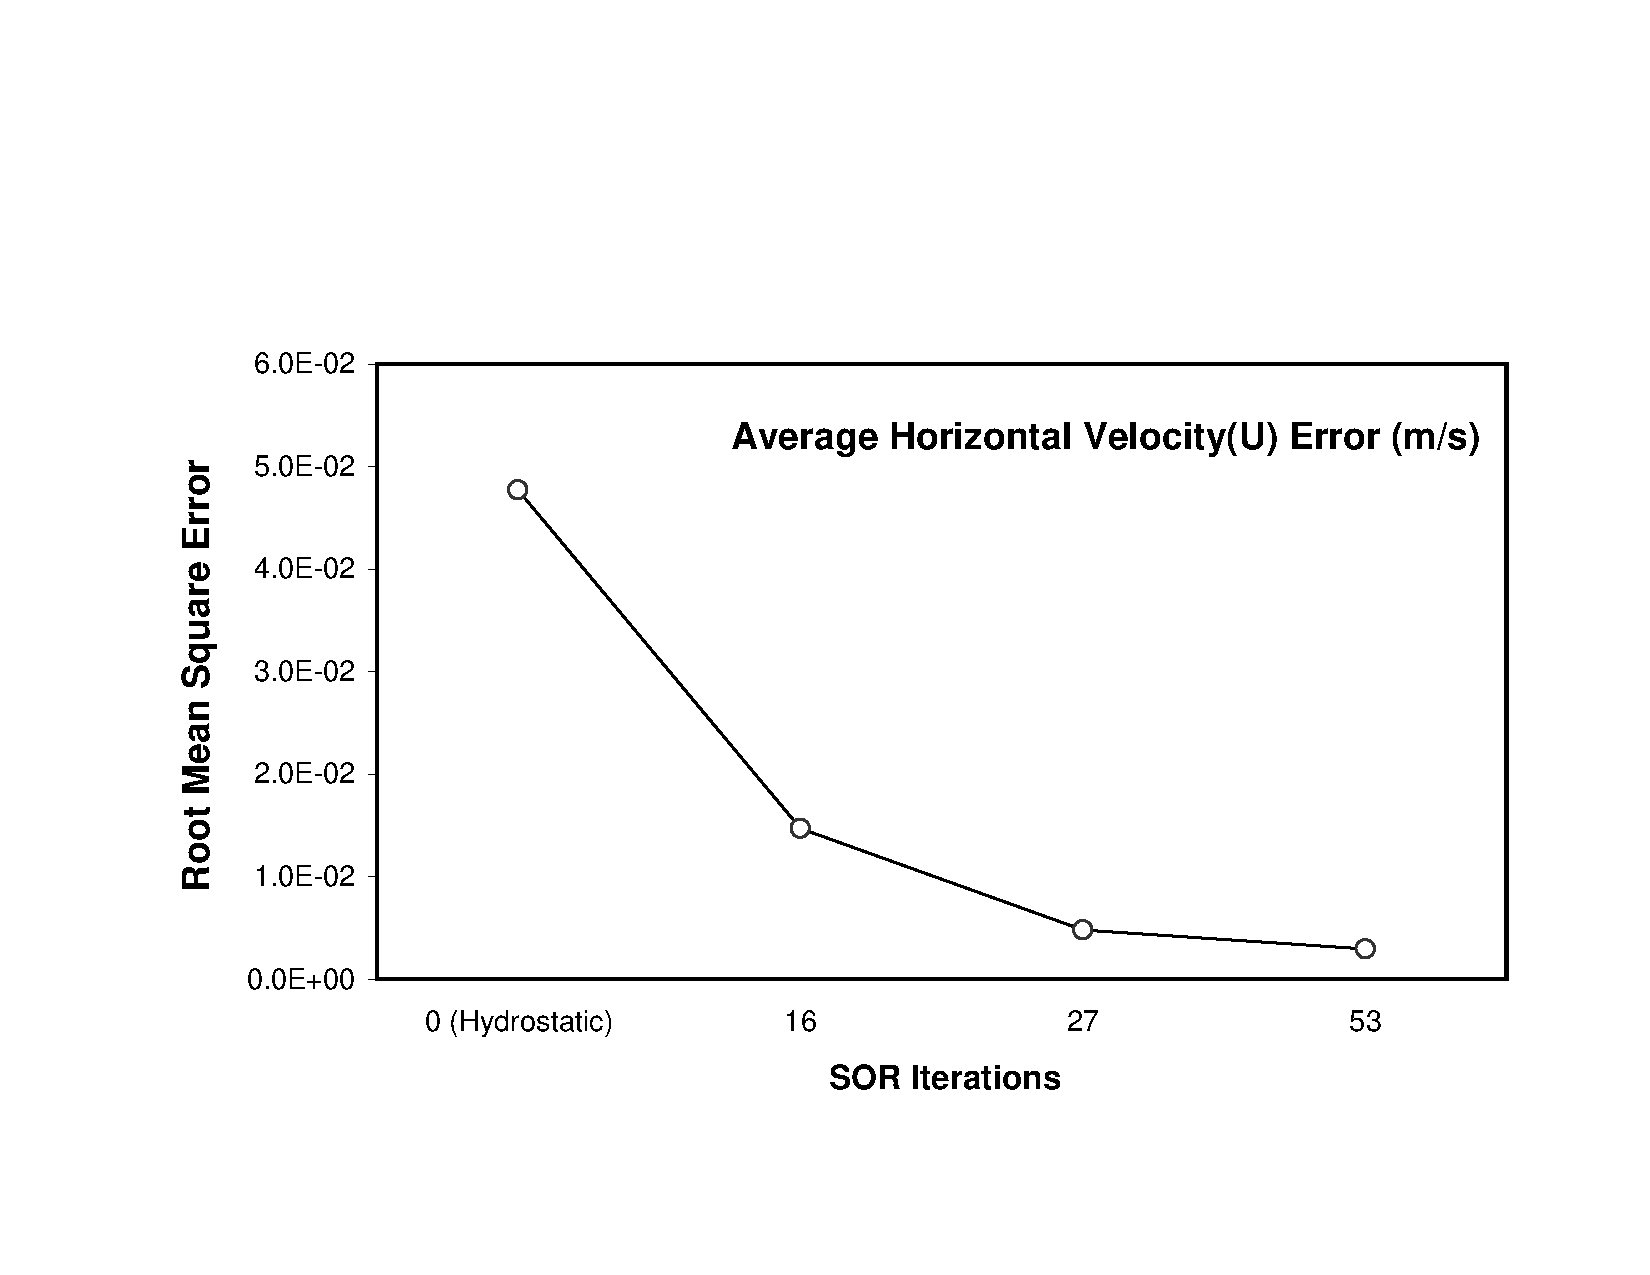
\includegraphics[width=4.0in]{../figures/ANH/2D_NX140/U.pdf}

\hspace{0.7in} \vspace{0.3in}
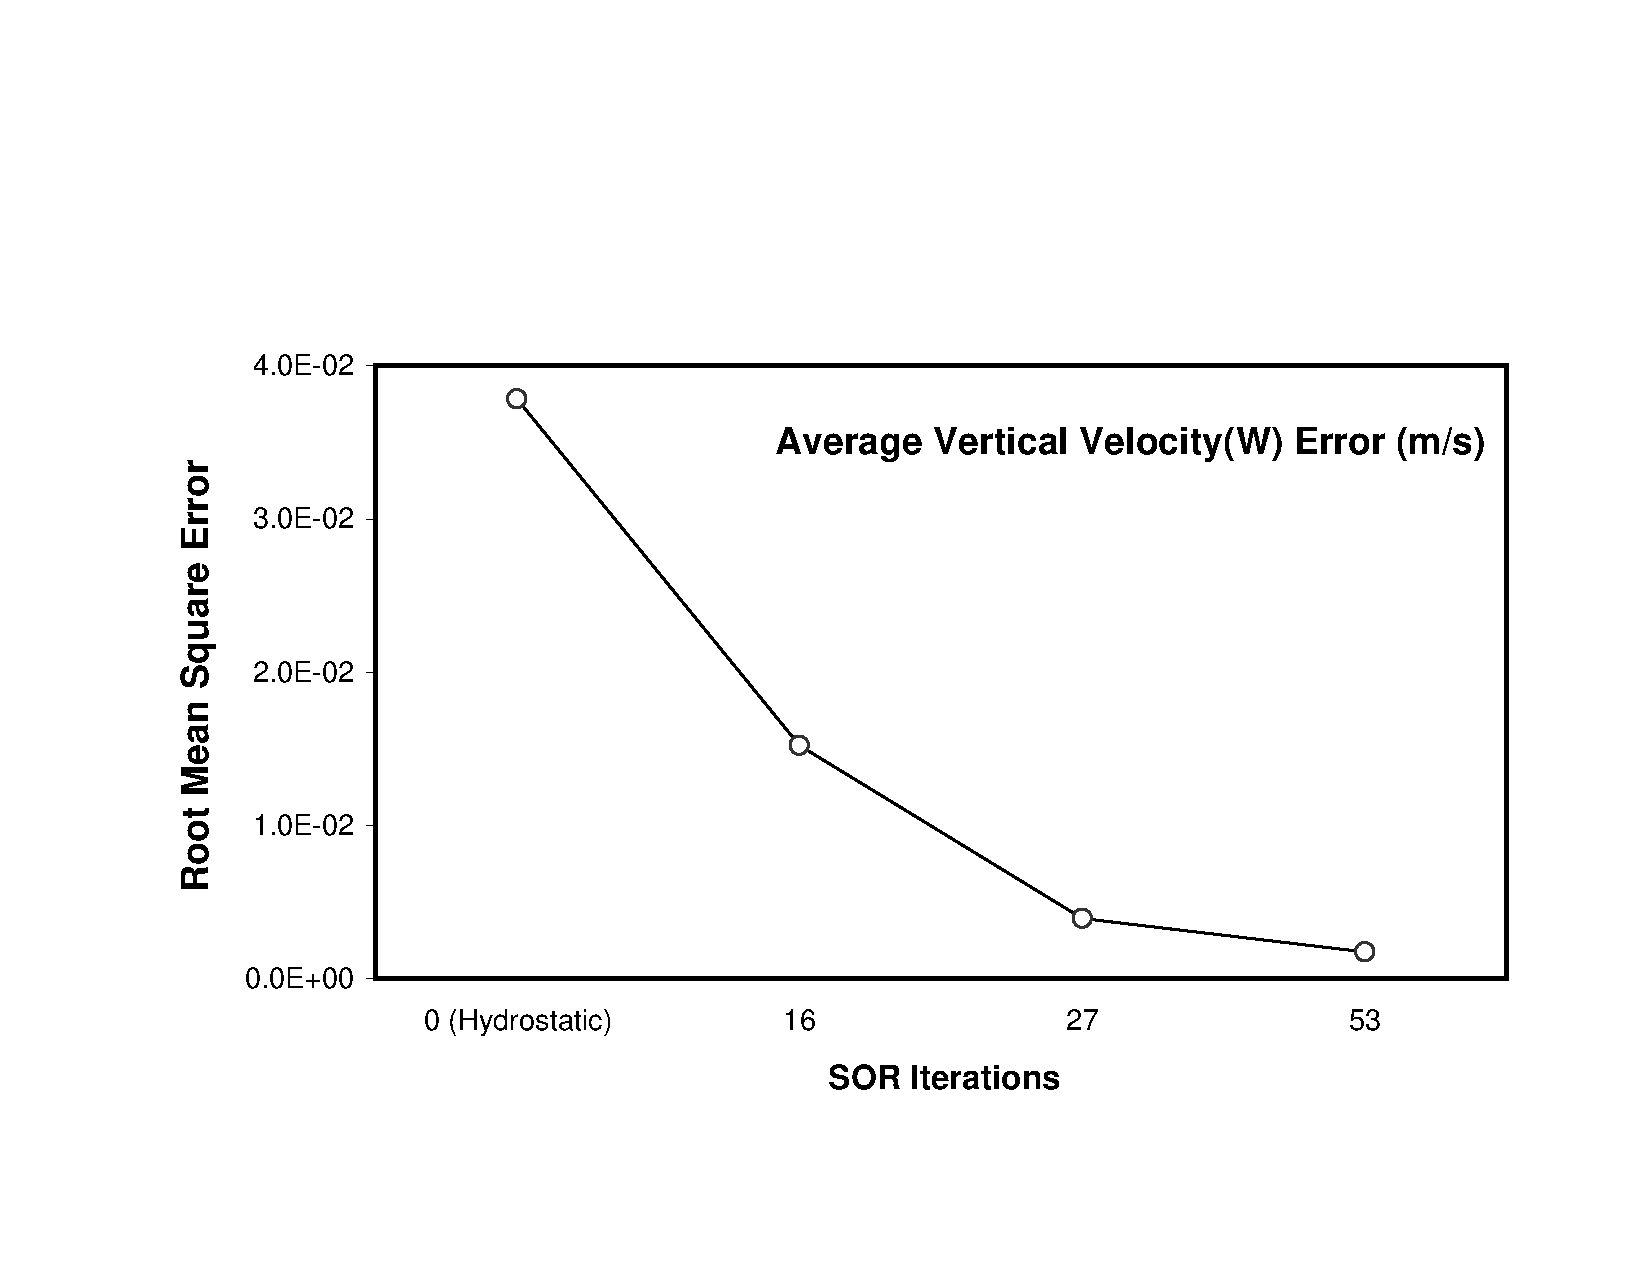
\includegraphics[width=4.0in]{../figures/ANH/2D_NX140/W.pdf}
\caption{Average errors for two dimensional gravity current simulations with different average SOR iterations resulted from different stopping criteria for the solution of pressure Poisson equation.}
\label{fig:ANH-summary-2D-error}
\end{figure}

\cp
